%%%%%%%%%%%%%%%%%%%%%%%%%%%%%%%%%%%%%%%%%%%%%%%%%%%%%%%%%%%%%%%%%%%%%%%%%%%%%
%%                                                                         %%
%%                   LaTeX Vorlage für die Studenten der                   %%
%%              Dualen Hochschule Baden-Württemberg Ravensburg             %%
%%                                                                         %%
%%  Die Vorlage orientiert sich an den Gestaltungsrichtlinien der DHBW RV  %%
%%                                                                         %%
%%                                                                         %%
%% Ersteller:        Markus Schutz (WI06)                                  %%
%% letzten Änderung: 26. November 2013                                     %%
%%                                                                         %%
%%                                                                         %%
%% Wichtiger Hinweis:                                                      %%
%%                                                                         %%
%% Keine Änderungen an den Dateien im Verzeichnis "pages" vornehmen. Für   %%
%% die Arbeit beziehen sich alle Änderungen auf diese Datei und die        %%
%% Dateien im Verzeichnis "chapter".                                       %%
%% Für die Erstellung des Literaturverzeichnises empfiehlt sich die Ver-   %%
%% wendung von JabRef (http://jabref.sourceforge.net). Die Datei ist unter %%
%% dem Namen literatur.bib im Verzeichnis "literatur" zu speichern.        %%
%%                                                                         %%
%% Zur sinnvollen Nutzung dieser Vorlage empfiehlt es sich, die Dokus zu   %%
%% den eingebundenen Paketen durchzulesen. Sie sind im doc-Verzeichnis der %%
%% MiKTeX-Installation zu finden.                                          %%
%%                                                                         %%
%% Enthaltene Titelblätter:                                                %%
%%   - Seminararbeit                                                       %%
%%   - Projektarbeit                                                       %%
%%   - Bachelorarbeit                                                      %%
%%                                                                         %%
%%%%%%%%%%%%%%%%%%%%%%%%%%%%%%%%%%%%%%%%%%%%%%%%%%%%%%%%%%%%%%%%%%%%%%%%%%%%%

\documentclass[a4paper,12pt]{article}                                         % Schriftgröße, Layout, Papierformat, Art des Dokumentes
\usepackage[left=3cm,right=2cm,top=2cm,bottom=2cm,includehead]{geometry}      % Einstellungen der Seitenränder
\usepackage[ngerman]{babel}                                                   % deutsche Silbentrennung
\usepackage[utf8]{inputenc}                                                   % Umlaute
\usepackage[hyperfootnotes=false, hidelinks=true]{hyperref}                                   % pfd-Output [Fußnoten nicht verlinken]
\usepackage[nottoc]{tocbibind}                                                % Inhaltsverzeichniserweiterung (Inhaltsverzeichnis selbst ausblenden)
\usepackage{makeidx}                                                          % Index
\usepackage[intoc]{nomencl}                                                   % Abkürzungsverzeichnis
\usepackage{fancyhdr}                                                         % Fancy Header
\usepackage[round]{natbib}                                                    % Zitate (Erweiterung für Literaturverzeichnis)
\usepackage{amsmath}                                                          % Zurücksetzen der Tabellen- und Abbildungsnummerierung je Sektion
\usepackage[labelfont=bf,aboveskip=1mm]{caption}                              % Bild- und Tabellenunterschrift (fett)
\usepackage{setspace}                                                         % Zeilenabstand (vor footmisc laden!)
\usepackage[bottom,multiple,hang,marginal]{footmisc}                          % Fußnoten [Ausrichtung unten, Trennung durch Seperator bei mehreren Fußnoten]
\usepackage{graphicx}                                                         % Grafiken
\usepackage{tabularx}                                                         % erweiterte Tabellen
\usepackage{longtable}                                                        % mehrseitige Tabellen
\usepackage{color}                                                            % Farben
\usepackage{enumitem}                                                         % Befehl setlist (Zeilenabstand für itemize Umgebung auf 1 setzen)
\usepackage{listings}                                                         % Quelltexte
\usepackage{zref}                                                             % Verweise (Anhangsverweise)
\usepackage[toc,style=altlist,translate=false]{glossaries}                    % Glossar (nach hyperref, inputenc, babel und ngerman)
\usepackage{glossaries-babel}                                                 % Glossar: Übersetzung im TOC
\usepackage{lipsum}
\usepackage{float}
\usepackage{listing}
\usepackage{pdfpages}


%%%%%%%%%%%%%%%%%%%%%%%%%%%%%%%%%%%%%%%%%%%%%%%%%%%%%%%%%%%%%%%%%%%%%%%%%%%%%
%%                                                                         %%
%% \/   \/      Bitte hier die Änderungen zur Arbeit vornehmen     \/   \/ %%
%%                                                                         %%
%%%%%%%%%%%%%%%%%%%%%%%%%%%%%%%%%%%%%%%%%%%%%%%%%%%%%%%%%%%%%%%%%%%%%%%%%%%%%

%%%%%%%%%%%%%%%%%%%%%%% Definitionen bzgl. der Arbeit %%%%%%%%%%%%%%%%%%%%%%%
\def\myType{0}           % [0=Seminararbeit|1=Projektarbeit|2=Bachelorarbeit]

\def\myTopic{Ant Colony Optimization }
\def\mySubTopic{(Ameisen-Algorithmen)}
\def\myAutor{Felix Behne, Moritz Link, Markus Koch, Sarah Engelmayer}
\def\myProf{Herr Timo Buck}
\def\myEndDate{25.06.2021}

%%%%%%%%%%%%%%%%%%%% Folgende Angaben für: Seminararbeit %%%%%%%%%%%%%%%%%%%%
\def\myVorlesung{Applied Optimization Techniques}

%%%%%%%%%%%%%%%%%%%% Folgende Angaben für: Projektarbeit %%%%%%%%%%%%%%%%%%%%
\def\myProjNumber{Nummer der Projektarbeit}         % [1|2]
\def\myPraxPhase{Studienjahr}                       % [1|2|3]

%%%%%%%%%%%%%%%%%%%%%%%%%%%%%%%%%%%%%%%%%%%%%%%%%%%%%%%%%%%%%%%%%%%%%%%%%%%%%
%%                                                                         %%
%% /\   /\         Ab hier keine Änderungen mehr vornehmen         /\   /\ %%
%%                                                                         %%
%%%%%%%%%%%%%%%%%%%%%%%%%%%%%%%%%%%%%%%%%%%%%%%%%%%%%%%%%%%%%%%%%%%%%%%%%%%%%

%%%%%%%%%%%%%%%%%%%%%%%% Eigene Farbwerte definieren %%%%%%%%%%%%%%%%%%%%%%%%
\definecolor{boxgray}{gray}{0.9}         % Hintergrundfarbe für Zitatboxen
\definecolor{commentgray}{gray}{0.5}     % Grau für Kommentare in Quelltexten
\definecolor{darkgreen}{rgb}{0,.5,0}     % Grün für Strings in Quelltexten

%%%%%%%%%%%%%%%%%%%%%%%% Eigene Kommandos definieren %%%%%%%%%%%%%%%%%%%%%%%%
% Definition von \gqq{#1: text}: Text in Anführungszeichen
\newcommand{\gqq}[1]{\glqq #1\grqq}

% Definition von \footref{#1: label}
% Verweis auf bereits existierende Fußnoten mittels
\providecommand*{\footref}[1]{
	\begingroup
		\unrestored@protected@xdef\@thefnmark{\ref{#1}}
	\endgroup
\@footnotemark}

% Definition von \mypageref{#1: label}
% Kombination aus \ref{#1: label} und \pageref{#1: label}
\newcommand{\mypageref}[1]{\ref{#1} auf Seite \pageref{#1}}

% Definition von \myboxquote{#1: text}
% grau hinterlegte Quotation-Umgebung (für Zitate)
\newcommand{\myboxquote}[1]{
	\begin{quotation}
		\colorbox{boxgray}{\parbox{0.78\textwidth}{#1}}
	\end{quotation}
	\vspace*{1mm}
}

\makeatletter
\zref@newprop*{appsec}{}
\zref@addprop{main}{appsec}

% Definition von \applabel{#1: label}{#2: text}
% von \appsec{#1: text}{#2: label} zur Erzeugung des Labels verwendet)
\def\applabel#1#2{%
	\zref@setcurrent{appsec}{#2}%   
	\zref@wrapper@immediate{\zref@label{#1}}%
}

% Definition von \appref{#1: label}
% anstelle \ref{#1: label} zum referenzieren von Anhängen verwenden)
\def\appref#1{%
	\hyperref[#1]{\zref@extract{#1}{appsec}}%
}
\makeatother

% Definition von \appsection{#1: text}{#2: label}
% Ersetzt \section{#1: text} und \label{#2: label} für Anhänge)
\newcommand{\theappsection}[1]{Anhang \Alph{section}:~\protect #1}
\newcommand{\appsection}[2]{
	\addtocounter{section}{1}
	\phantomsection
	\addcontentsline{toc}{section}{\theappsection{#1}}
	\markboth{\theappsection{#1}}{}

	\section*{\theappsection{#1}}
	\applabel{#2}{Anhang \Alph{section}}
	\label{#2}
}

%%%%%%%%%%%%% Index, Abkürzungsverzeichnis und Glossar erstellen %%%%%%%%%%%%
\makeindex
\makenomenclature
\makeglossaries

% Festlegung der Art der Zitierung (Havardmethode: Abkuerzung Autor + Jahr) %
\bibliographystyle{dinat}

%%%%%%%%%%%%%%%%%%%%%%%%%%%%%%% PDF-Optionen %%%%%%%%%%%%%%%%%%%%%%%%%%%%%%%%
\hypersetup{
	bookmarksopen=false,
	bookmarksnumbered=true,
	bookmarksopenlevel=0,
	pdftitle=\myTopic,
	pdfsubject=\myTopic,
	pdfauthor=\myAutor,
	pdfstartview=Fit,
	pdfpagelayout=SinglePage
}

%%%%%%%%%%%%%%%%%%%%%%%%%%%% Kopf- und Fußzeile %%%%%%%%%%%%%%%%%%%%%%%%%%%%%
\pagestyle{fancy}
\fancyhf{}
\fancyhead[R]{\thepage}                         % Kopfzeile rechts bzw. außen
\renewcommand{\headrulewidth}{0.5pt}            % Kopfzeile rechts bzw. außen

%%%%%%%%%%%%%%%%%%%%%%%%% Layout und Beschriftungen %%%%%%%%%%%%%%%%%%%%%%%%%
\onehalfspacing                % Zeilenabstand: 1.5 (Standard: 1.2)
\setlist{noitemsep}            % Zeilenabstand für items auf 1 setzen

\addto\captionsngerman{        % Tabllen- und Abbildungsunterschriften ändern
  \renewcommand{\figurename}{Abb.}
  \renewcommand{\tablename}{Tab.}
}
\numberwithin{table}{section}                               % Tabellennummerierung je Sektion zurücksetzen
\numberwithin{figure}{section}                              % Abbildungsnummerierung je Sektion zurücksetzen
\renewcommand{\thetable}{\arabic{section}.\arabic{table}}   % Tabellennummerierung mit Section
\renewcommand{\thefigure}{\arabic{section}.\arabic{figure}} % Abbildungsnummerierung mit Section
\renewcommand{\thefootnote}{\arabic{footnote}}              % Sektionsbezeichnung von Fußnoten entfernen

\renewcommand{\multfootsep}{, }                             % Mehrere Fußnoten durch ", " trennen

%%%%%%%%%%%%%%%%%%%%%%%%%%%%%%% Listingstyle %%%%%%%%%%%%%%%%%%%%%%%%%%%%%%%%
\lstset{
	basicstyle=\ttfamily\scriptsize,
	commentstyle=\color{commentgray}\textit,
	showstringspaces=false,
	stringstyle=\color{darkgreen},
	keywordstyle=\color{blue},
	numbers=left,
	numberstyle=\tiny,
	stepnumber=1,
	numbersep=15pt,
	tabsize=2,
	fontadjust=true,
	frame=single,
	backgroundcolor=\color{boxgray},
	captionpos=b,
	linewidth=0.94\linewidth,
	xleftmargin=0.1\linewidth,
	breaklines=true,
	aboveskip=16pt
}
        
%%%%%%%%%%%%%%%%%%%%%%%%%%%%%%%%%%%%%%%%%%%%%%%%%%%%%%%%%%%%%%%%%%%%%%%%%%%%%
%%                                                                         %%
%% \/   \/      Bitte hier die Änderungen zur Arbeit vornehmen     \/   \/ %%
%%                                                                         %%
%%%%%%%%%%%%%%%%%%%%%%%%%%%%%%%%%%%%%%%%%%%%%%%%%%%%%%%%%%%%%%%%%%%%%%%%%%%%%

%Seiten und Kapitel einbinden
\begin{document}
	\pagenumbering{Roman}
	% Das Titelblatt wird automatisch ausgewählt. Keine Änderung hier
	\ifcase\myType
		\begin{titlepage}
	\begin{center}
		\vspace*{2cm}
		\LARGE\bf\myTopic\\
		\Large\rm\mySubTopic\\
		\vspace*{3cm}
		\bf Seminararbeit zur Vorlesung\\
		\myVorlesung\\
		\normalsize\rm
		\vspace*{1cm}
		für die\\
		Prüfung zum Bachelor of Science\\
		\vspace*{1cm}
		an der Fakultät für Wirtschaft\\
		im Studiengang Wirtschaftsinformatik\\
		\vspace*{1cm}
		an der\\
		DHBW Ravensburg
		\vfill
	\end{center}
	\begin{tabular}{ll}
		Verfasser:&\myAutor\\
		Wiss. Betreuer:&\myProf\\
		Abgabedatum:&\myEndDate\\
	\end{tabular}
\end{titlepage}
\newpage
\setcounter{page}{2}

	\or
		\begin{titlepage}
	\begin{center}
		\vspace*{1cm}
		\LARGE\bf\myTopic\\
		\Large\rm\mySubTopic\\
		\vspace*{2cm}
		\bf \myProjNumber.~Projektarbeit\\
		\vspace*{1cm}
		\normalsize\rm
		Praxisphase des \myPraxPhase. Studienjahrs \\
		\vspace*{1cm}
		an der Fakultät für Wirtschaft\\
		im Studiengang Wirtschaftsinformatik\\
		\vspace*{1cm}
		an der\\
		DHBW Ravensburg
		\vfill
	\end{center}
	\begin{tabular}{ll}
		Verfasser:&\myAutor\\
		Ausbildungsbetrieb:&\myCompany\\
		Anschrift:&\myCompanyAddressStreet\\
		&\myCompanyAddressCity\\
		Wiss. Betreuer:&\myProf\\
		Abgabedatum:&\myEndDate\\
	\end{tabular}
	\newline
	\vspace*{1cm}
	\newline
	\begin{tabularx}{\textwidth}{l@{\extracolsep\fill}r}
	  Unterschrift des verantwortlichen Ausbilders&\\
	  (oder des Personalverantwortlichen)&\rule{6cm}{0.3mm}\\
	\end{tabularx}
\end{titlepage}
\newpage
\setcounter{page}{2}

	\or
		\begin{titlepage}
	\begin{center}
		\vspace*{2cm}
		\LARGE\bf\myTopic\\
		\Large\rm\mySubTopic\\
		\vspace*{3cm}
		\bf Bachelorarbeit\\
		\normalsize\rm
		\vspace*{1cm}
		für die\\
		Prüfung zum Bachelor of Science\\
		\vspace*{1cm}
		an der Fakultät für Wirtschaft\\
		im Studiengang Wirtschaftsinformatik\\
		\vspace*{1cm}
		an der\\
		DHBW Ravensburg
		\vfill
	\end{center}
	\begin{tabular}{ll}
		Verfasser:&\myAutor\\
		Ausbildungsbetrieb:&\myCompany\\
		Anschrift:&\myCompanyAddressStreet\\
		&\myCompanyAddressCity\\
		Wiss. Betreuer:&\myProf\\
		Abgabedatum:&\myEndDate\\
	\end{tabular}
\end{titlepage}
\newpage
\setcounter{page}{2}

	\else
	\fi
	
	\pagestyle{fancy}
	\tableofcontents
\newpage

	\renewcommand{\nomname}{Abkürzungsverzeichnis}
\setlength{\nomlabelwidth}{.25\hsize}
\renewcommand{\nomlabel}[1]{#1 \dotfill}
\setlength{\nomitemsep}{-\parsep}
\printnomenclature
\newpage

	% \renewcommand{\glossaryname}{Glossar}
\printglossaries
	\listoffigures
\newpage

	% \listoftables
\newpage


	% Kapitel
	\pagestyle{fancy}
	\fancyhead[L]{\nouppercase{\leftmark}}                               % Kopfzeile links bzw. innen
	\pagenumbering{arabic}
	\section{Einleitung}\label{chap:Einleitung}

Logistikunternehmen, Busunternehmen oder die Müllabfuhr stehen täglich vor dem Problem, alle geplanten Zielstationen in möglichst kurzer Zeit, mit möglichst geringem Treibstoffverbrauch und unter Berücksichtigung weiterer Nebenbedingungen anzufahren.\newline     
In dieser Arbeit soll das Optimierungsverfahren Ant Colony Optimization (ACO)\nomenclature{\(ACO\)}{Ant Colony Optimization}, das u.A. für die Routenoptimierung eingesetzt wird, vorgestellt werden. \newline
Um Inhalte anschaulich und interaktiv veranschaulichen zu können, wurde hierfür ein Dashboard mittels R-Shiny erstellt. \newline
Ziel dieses Projektberichts ist es, den Quellcode des Dashboards zu erläutern sowie den Aufbau, die Inhalte und die Auswahl der Elemente des R-Shiny-Dashborads zu beschreiben und zu begründen. \newline
Hierbei wird zunächst auf die Struktur des Dashboards eingegangen. Weiterhin wird erläutert, wie allgemeine Informationen zu ACO im Dashboard dargestellt werden. Anschließend wird erläutert, wie die Vorgehensweise des Algorithmus  im R-Shiny Dashboard unter Verwendung interaktiver Elemente visualisiert wird. Weiterhin wird das im Dashboard dargestellte Problem des Handlungsreisenden als Anwendungsgebiet des Algorithmus erläutert und die Umsetzung eines Performance-Vergleichs mit anderen Algorithmen im Dashboard erläutert. 
Zuletzt werden Inhalte und gewonnene Erkenntnisse in einem Fazit zusammengefasst. 
	\section{Aufbau und Organisation des Dashboards}

\subsection{\{Golem\}}\label{chap:Golem}
\{Golem\} ist ein R-Paket, welches es erleichtert skalierbare und standardisierte Shiny-Applikationen zu bauen. Es ist Teil des golemverse und seit dem 05 August 2019 auf dem \glqq Comprehensive R Archive Network\grqq{} (CRAN) \nomenclature{\(CRAN\)}{Comprehensive R Archive Networks} gehosted \citep{ThinkR2019}.\newline
Das golemverse \citep{ThinkRnodate} ist eine Sammlung verschiedener R-Pakete, welche die Entwicklung von Shiny Dashboards beschleunigen sollen. Es wurde von dem französischen Consulting Unternehmen ThinkR \citep{Breizhtormnodate} entwickelt.\newline
ThinkR ist ein Consulting Unternehmen, welches sich auf das Ausrichten von interaktiven Trainings im Bereich der R Programmierung, mit einem Fokus auf die Entwicklung von Shiny Dashboards, spezialisiert hat. \newline
{Golem} folgt dem Grundatz \glqq convention over configuration\grqq{}. 
Einem Softwaredesign-Paradigma, welches in seiner Grundidee von David Heinemeier Hansson \citep{Hansson2016} für das Web-Framework \glqq Ruby on Rails\grqq{} entwickelt wurde. Dabei steht im Zentrum des Paradigmas die Idee, mit Konventionen die Anzahl der Entscheidungen, die ein Programmierer zu treffen hat, zu reduzieren. Dies führt zu einer hohen Softwarequalität, bei veringertem Aufwand für den Programmierer. \newline
In \{golem\} wird das durch eine vordefinierte Ordnerstruktur, zentrale Konfigurationsdateien und Funktionen zum Erstellen neuer Teile des Dashboards umgesetzt. \newline 
Dieser Ansatz hat den Vorteil, dass er das Team zu einer hohen Softwarequalität zwingt. \newline 
Im Folgenden, sollen die einzelnen Komponenten von \{golem\} näher erläutert und deren Wichtigkeit herausgestellt werden.

\begin{figure}
 \centering
 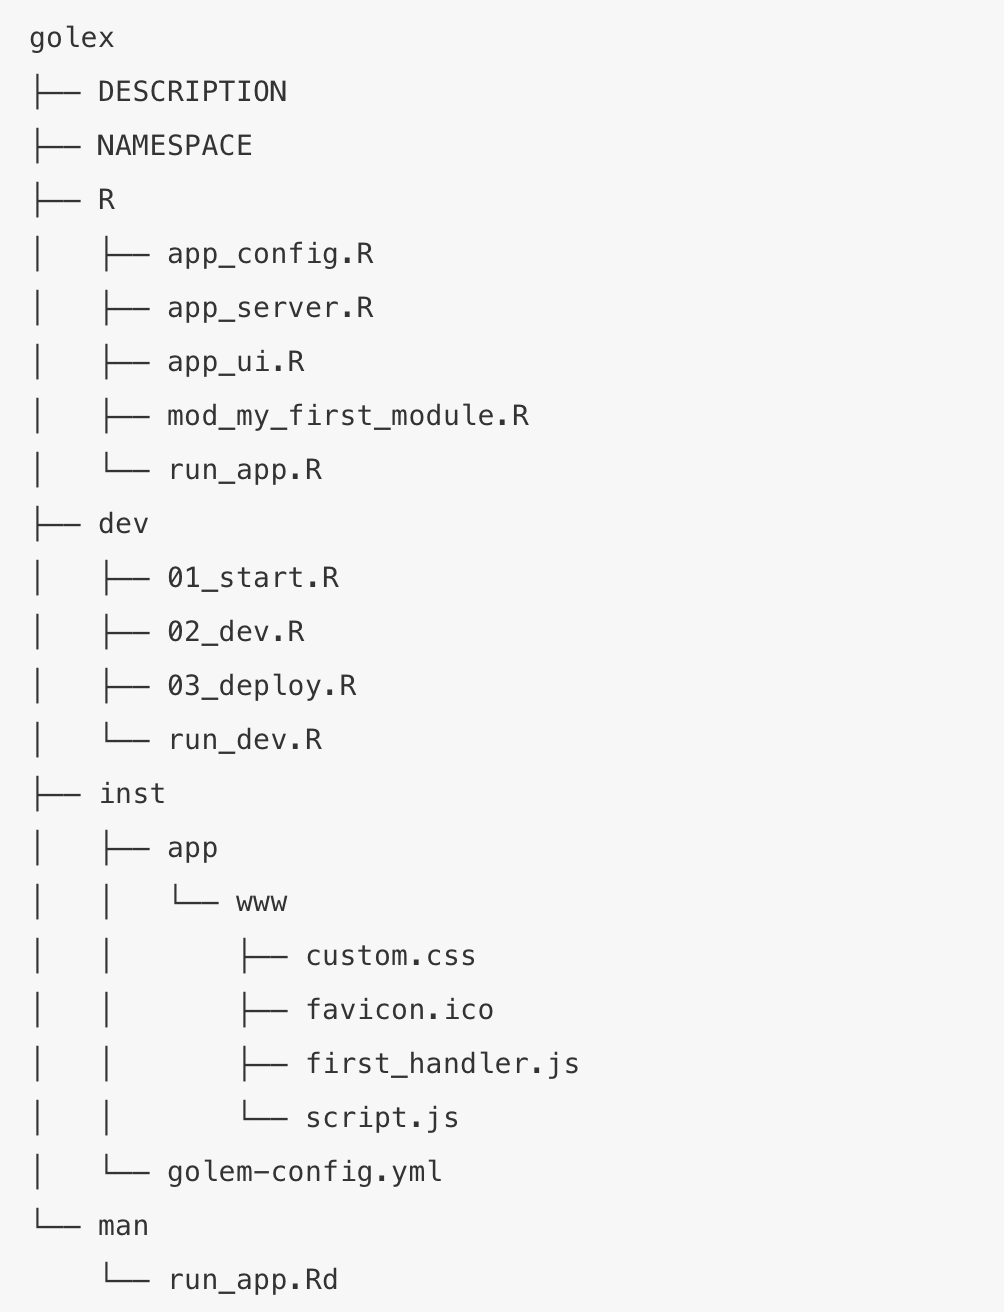
\includegraphics[scale=.4]{"images/02_Aufbau_und_Organisation/golem_app_structure.png"}
 \caption{Golem App Struktur}
\end{figure}

\subsubsection{DESCRIPTION und NAMESPACE}
Die DESCRIPTION und NAMESPACE Dateien enthalten Metadaten über das Package und sind nicht \{golem\} spezifisch.\newline 
Bei der Erstellung eines \{golem\} Projekts werden diese Dateien automatisch generiert und in der Regel bedarf es keiner manuellen Änderungen. \newline
Die DESCRIPTION Datei enthält dabei unter Anderem Daten über die Funktionen des Packages, die Lizenz, die Autoren etc.. \newline
Die NAMESPACE Datei definiert wie Interaktionen mit anderen Paketen aussehen. Dabei wird betrachtet, welche Funktionen von dem Package importiert und exportiert werden.\newline
Um eine lückenlose Dokumentation zu gewährleisten und mögliche Fehler zu vermeiden, sollte diese Datei niemals per Hand bearbeitet werden. Um Änderungen an der Datei vorzunehmen, kann das Paket \emph{attachment} \citep{Rochette2021} verwendet werden. Dieses updated, basierend auf \emph{@import} und \emph{@export} Tags in den Docstrings der einzelnen Funktionen und Modulen, die NAMESPACE Datei.
Ein solches Update kann manuell mit folgendem Command getriggert werden:
\begin{lstlisting}
attachment::att_amend_desc()
\end{lstlisting}

\subsubsection{R/}
Dieser Ordner enthält den Kern-Quellcode einer \{golem\} Applikation. 
Nach der initialen Erstellung eines \{golem\} Projekts, befinden sich vier Dateien in dem Ordner: app\_config.R, app.R, ui.R und server.R. \newline 
Die app\_config.R Datei ist \{golem\} spezifisch und enthält Konfigurationsparameter.\newline 
Die app.R Datei führt die Server-und die Ui-Funktionen zu einem Dashboard zusammen und enthält zudem \{golem\} spezifische Funktionsaufrufe. \newline 
Die ui.R Datei enthält die Definition des User-Interface der Applikation und die server.R Datei definiert die Backend-Logik, welche auf dem Server und nicht im Browser läuft.

\subsubsection{dev/}
Der dev Ordner enthält \{golem\} spezifische Utility-Funktionen, welche z.B. das Deployment der App vereinfachen. Dieser Ordner enthält keinen applikationsspezifischen Code. 

\subsubsection{inst/app/www}
Der inst/app/www Ordner enthält statische Dateien, wie z.B. Bilder oder CSS Dateien. Alle Dateien, die in diesem Ordner abgelegt werden, stehen der Applikation bei Laufzeit zur Verfügung. 

\subsection{Aufbau des Dashboards}\label{chap:Aufbau}
 Das Shiny-Dashboard startet auf der Welcomepage, wo die vier Bereiche App Status, App Mainteners, Directions und Security and License vorgefunden werden können:
\begin{figure} [H]
 \centering
 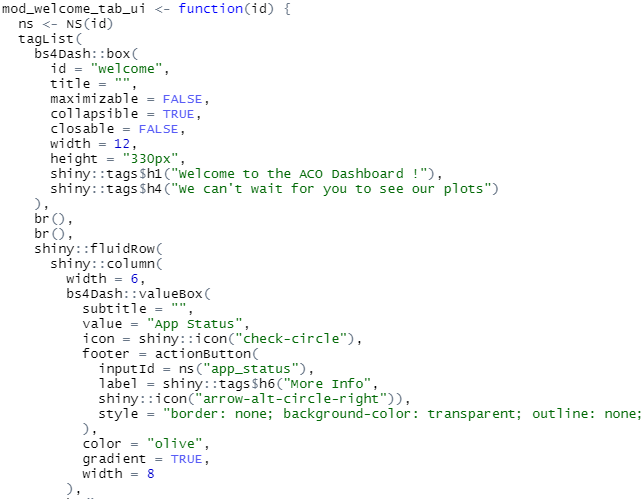
\includegraphics[scale=.8]{"images/02_Aufbau_und_Organisation/ui_welcomepage.png"}
 \caption{Quellcode des UI Funktion für die WelcomePage}
 \label{fig:fluidPage}
\end{figure}

Jeder Tab entspricht einem Shiny-Module. Diese Vorgehensweise reduziert Namespace Konflikte und entspricht den Best Practices von \{golem\}.\newline
Die Tabs selber werden in dem Dashboard auf der linken Seite abgebildet. Hierzu werden die Tabs aufgeklappt, sobald man mit dem Mauscursor über die Fläche fährt. Es gibt eine Aufteilung in Welcome, welches die WelcomePage beinhaltet, desweiteren gibt es den übergeordneten Punkt Theoretical Background, in dem die Themen Timeline, Ant Foraging und Algorithm untergebracht wurden. Der nächste übergeordnete Punkt sind Visualisations unter dem der Ant Generations Plot, Rosenbrock Plot und Himmelblau Plot vorliegt. Als letzter übergeordneter Punkt wurde Applying the algorithm verwendet, welcher das Travelling Salesman Problem und den Performancevergleich zu anderen Algorithmen beinhaltet. \newline
Die Implementierung des ACO im Algorithm Tab basiert auf dem Artikel: \glqq \emph{Ant Colony Optimization Algorithm}\grqq{} von Pablo Portillo Garrigues \citep{Garrigues2019}.
	\include{projektarbeit-ant-colony-optimization/chapter/03_Theoretische_Hintergründe}
	\section{Visualisierung des Algorithmus} \label{chap:Visualisierung}


Ein Seiten-Tab-Reiter des R-Shiny-Dashboards, wird der Visualisierung des Algorithmus gewidmet. 
Dieser besteht aus drei Unter-Reitern, in denen Generationen von Ameisen visuell gezeigt werden und der Algorithmus auf die Rosenbrock- und auf die Himmelblaufunktion angewendet wird. Den zugehörigen Quellcode-Ausschnitt der app\_ui.R Datei zeigt Abbildung \ref{fig:app_ui_visualisations_tab}. 

\begin{figure}[H]
 \centering
 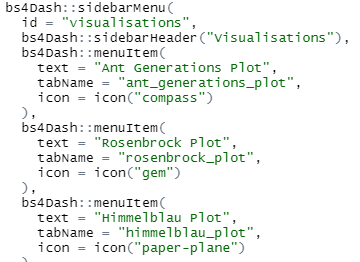
\includegraphics[scale=1]{"images/04_Visualisierung_des_Algorithmus/app_ui_visualisations_tab.png"}
 \caption{Quellcode in app\_ui.R zur Darstellung des seitlichen Navigation-Tab-Reiters für Visualisierungen des ACO}
 \label{fig:app_ui_visualisations_tab}
\end{figure}

In den beiden Unter-Reitern \textit{Rosenbrock Plot} und \textit{Himmelblau Plot} werden die Optimierungsfunktionen jeweils in einem 3d-Plot dargestellt. Die Funktion, die diesen Graph generiert, zeigt Abbildung \ref{fig:util_3dplot}.
Dem Benutzer werden hierbei interaktive Schieberegler zur Veränderung der Darstellung des Plots in der rechten Seitenleiste zur Verfügung gestellt. Diese werden in Abbildung \ref{fig:ui_RoseHimPlot_2} dargestellt. 

\begin{figure}[H]
 \centering
 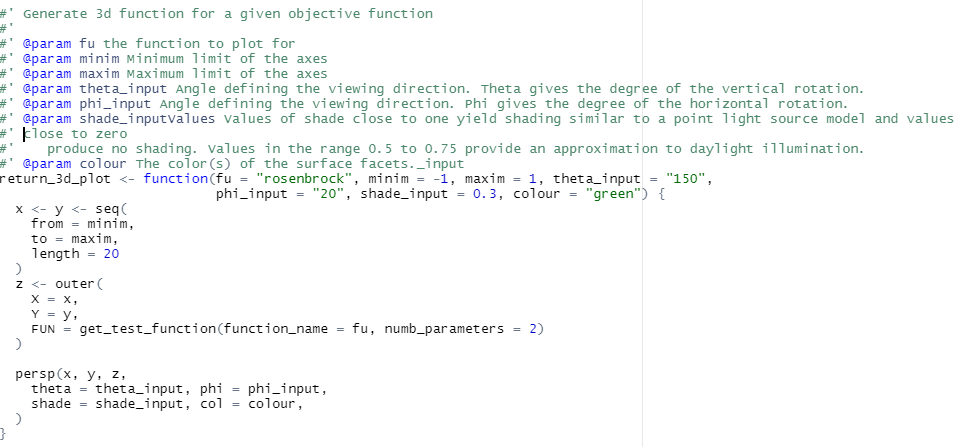
\includegraphics[scale=0.7]{"images/04_Visualisierung_des_Algorithmus/util_3dplot.png"}
 \caption{Funktion in global\_utils.R zur Generierung eines dreidimensionalen Graphen der Rosenbrock- oder Himmelblau-Funktion)}
 \label{fig:util_3dplot}
\end{figure}


\begin{figure}[H]
 \centering
 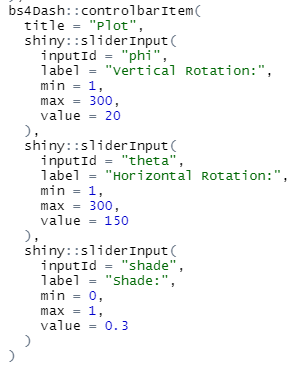
\includegraphics[scale=.7]{"images/04_Visualisierung_des_Algorithmus/ui_slider_for_rose_him_plots_2.png"}
 \caption{Quellcode in fct\_update\_controlbar.R zur Darstellung interaktiver Elemente für die Ansicht und Schattierung des drei-dimensionalen Graphen der Optimierungsfunktion (Rosenbrock oder Himmelblau-Funktion)}
 \label{fig:ui_RoseHimPlot_2}
\end{figure}

Weiterhin wird das tatsächliche Minimum der Rosenbrockfunktion in global\_utils.R, der Datei für globale Funktionen, berechnet und in Form eines Data-Frames gespeichert, um sie auf dem Dashboard in Form einer Tabelle darstellen zu können (siehe Abbildung \ref{fig:global_Mimima_Rose}). Die Minima der Himmelblau-Funktion werden ebenfalls in Form eines Data Frames gespeichert (siehe Abbildung \ref{fig:global_Mimima_Him}). Hierbei wird nur eines der Minima berechnet, während die weiteren drei Minima werden manuell hinzugefügt werden. 

\begin{figure}[H]
 \centering
 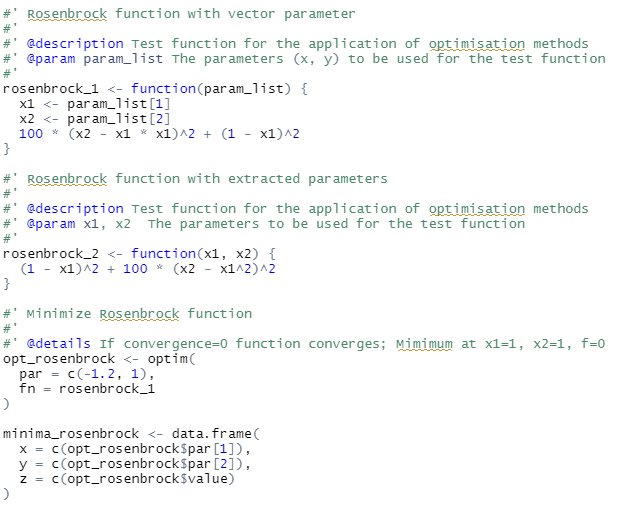
\includegraphics[scale=.7]{"images/04_Visualisierung_des_Algorithmus/utilsR_Minima_Rosenbrock.png"}
 \caption{Quellcode in global\_utils.R zur Erfassung und Speicherung des tasächlichen Minimums der Rosenbrock-Funktion}
 \label{fig:global_Mimima_Rose}
\end{figure}

\begin{figure}[H]
 \centering
 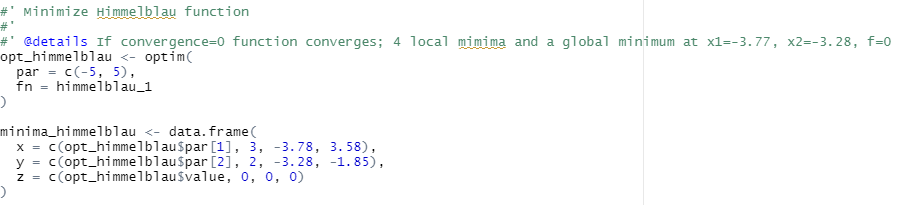
\includegraphics[scale=0.7]{"images/04_Visualisierung_des_Algorithmus/utilsR_Minima_Himmelblau.png"}
 \caption{Quellcode in global\_utils.R zur Speicherung der tasächlichen Minima der Himmelblaufunktion}
 \label{fig:global_Mimima_Him}
\end{figure}

Darüber hinaus sollen die tatsächlichen Minima der Optimierungsfunktionen mit den mittels ACO errechneten Minima verglichen werden können. 
Hierzu kann der Benutzer ebenfalls in Form von interaktiven Schiebereglern in den Algorithmus einfließende Parameter auswählen. Eine Veränderung dieser Parameter verursacht eine Änderung des anhand des Ameisenalgorithmus errechneten Ergebnisses.
Den zugehörigen Quellcode der fct\_update\_controlbar.R Datei zeigt Abbildung \ref{fig:ui_RoseHimPlot_1}.

\begin{figure}[H]
 \centering
 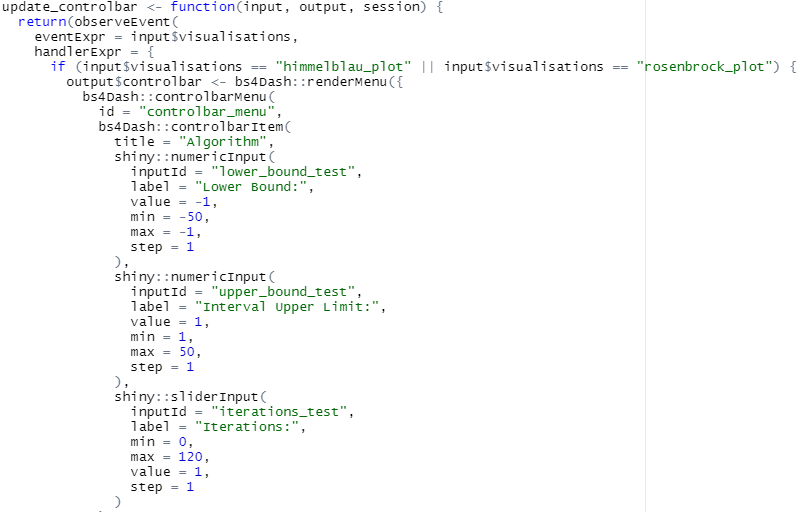
\includegraphics[scale=0.7]{"images/04_Visualisierung_des_Algorithmus/ui_slider_for_rose_him_plots_1.png"}
 \caption{Quellcode in fct\_update\_controlbar.R zur Darstellung interaktiver Elemente zur Festlegung des Such-Intervalls sowie der Anzahl an Iterationen zur Berechnung des Minimums mittels ACO}
 \label{fig:ui_RoseHimPlot_1}
\end{figure}

Um die Minima der Optimierungsfunktionen mittels ACO berechnen zu können, wird eine Funktion erstellt, welche in Abbildung \ref{fig:evoper_Minima_RoseHim_ACO} dargestellt wird. Hierbei wird das R-Package Evoper verwendet, das eine Implementierung des Ameisenalgorithmus beinhaltet. Die errechneten Minima werden neben den tatsächlichen Minima in einer zweiten Tabelle dargestellt und können so gut verglichen werden.
Sobald der Benutzer die Intervallgrenzen des Suchbereichs oder die Anzahl der Iterationen mithilfe der Schieberegler verändert, wird ein neues Ergebnis berechnet und die Tabelle der errechneten Minima wird aktualisiert. 
Je höher die Anzahl der Iterationen und je kleiner der Suchbereich, umso näher liegt das Ergebnis bei dem tatsächlichen Minimum bzw. an einem der tatsächlichen Minima. 
\newline
Bei der Himmelblaufunktion fällt auf, dass der Algorithmus bei Veränderung der Parameter maximal zwei der Minima findet. Unter welchen Voraussetzungen der Algorithmus in welches der Minima konvergiert, kann nicht festgelegt werden. Dies betont die Zuordnung des Ameisenalgorithmus zu den heuristischen Optimierungsverfahren, bei welchen unterschiedliche Start-Bedingungen zu unterschiedlichen Lösungen führen können. 

\begin{figure}[H]
 \centering
 \includegraphics[scale=0.7]{"images/04_Visualisierung_des_Algorithmus/evoper_calculate_Minimum_HimRose"}
 \caption{Quellcode in fct\_aco\_evoper.R um Minima der Rosenbrock- und Himmelblaufunktion mithilfe des ACO zu berechnen}
 \label{fig:evoper_Minima_RoseHim_ACO}
\end{figure}

 Den Quellcode der server-Funktion für die Generierung des dreidimensionalen Graphen der Rosenbrock-Funktion und der Tabellen für die tatsächlichen sowie mittels ACO errechneten Minima zeigt Abbildung \ref{fig:server_Minima_Rose_ACO}.

\begin{figure}[H]
 \centering
 \includegraphics[scale=.7]{"images/04_Visualisierung_des_Algorithmus/server_minima_rosenbrock"}
 \caption{Quellcode in mod\_rosenbrock\_tab.R um Rosenbrockfunktion darzustellen und Minimum mit Ergebnis des ACO zu vergleichen}
 \label{fig:server_Minima_Rose_ACO}
\end{figure}

Außerdem wird in mod\_rosenbrock\_tab.R und mod\_himmelblau\_tab.R jeweils ein Button erstellt, bei dessen Klick ein Popup erscheint, das die mathematische Formel der Rosenbrock bzw. der Himmelblau-Funktion darstellt. Wie dies in dem Tabreiter, der die Rosenbrock-Funktion darstellt, umgesetzt wird, zeigt Abbildung \ref{fig:server_mod_rosenbrock_tab_actionbutton}.

\begin{figure}[H]
 \centering
 \includegraphics{"images/04_Visualisierung_des_Algorithmus/server_mod_rosenbrock_tab_actionbutton"}
 \caption{Quellcode in mod\_rosenbrock\_tab.R um die Formel der Rosenbrock-Funktion in einem Popup darzustellen}
 \label{fig:server_mod_rosenbrock_tab_actionbutton}
\end{figure}

Mithilfe eines weiteren Info-Buttons in dem Navigations-Tab-Reiter, in welchem die Rosenbrock-Funktion visualisiert und optimiert wird, wird die Differenz des tatsächlichen Minimums zu dem mittels ACO berechneten Minimum dargestellt. Dies bewirkt, dass der Betrachter auf einen Blick die Qualität des berechneten Ergebnisses erkennt und die Verbesserung des Ergebnisses mit steigender Anzahl an Iterationen einfacher feststellen kann.  

Der dritte Tab-Reiter zur Visualisierung des Algorithmus hat das Ziel, dem Benutzer die iterative Näherung zum Minimum und die Zusammensetzung der errechneten Lösung aus den einzelnen Lösungen der Ameisen näher zu bringen. Hierfür wird die Himmelblau-Funktion als zu optimierende Funktion festgelegt. Interaktive Elemente ermöglichen es dem Benutzer erneut, den Suchbereich und die Anzahl an Iterationen, die der Algorithmus vornimmt, festzulegen. Zudem kann der Benutzer an dieser Stelle die Anzahl an Ameisen einer Generation festlegen. 
Das Minimum wird in diesem Fall nicht mithilfe des R-Pakets Evoper berechnet, sondern auf Basis der Implementierung von Garrigues \citep{Garrigues2019}, die in der Datei fct\_aco.R zu finden ist. Seine Funktionen werden in selbst erstellten Funktionen, die im Folgenden erläutert werden, aufgerufen und verwendet. 
Abbildung \ref{fig:makeStartGen} zeigt eine Deklaration der Funktionen, die initiale Ameisenwerte zufällig generieren unter Berücksichtigung der Anzahl der Ameisen sowie des Suchintervalls, das vom Benutzer festgelegt wurde.
In einer weiteren Funktion wird der eigentliche Iterationsschritt des Algorithmus durchgeführt und die neuen Positionen der Ameisen berechnet d.h. die neue Generation erstellt. Dies wird in Grafik \ref{fig:util_makeNewGen} abgebildet.


\begin{figure}[H]
 \centering
 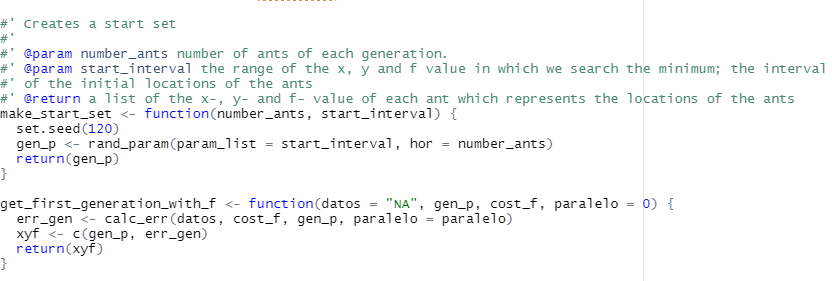
\includegraphics[scale=.7]{"images/04_Visualisierung_des_Algorithmus/util_makeStartGen.png"}
 \caption{Definition von Funktionen in global\_utils.R um Ameisengeneration zu initialisieren und Iterationsschritt durchzuführen}
 \label{fig:makeStartGen}
\end{figure}

\begin{figure}[H]
 \centering
 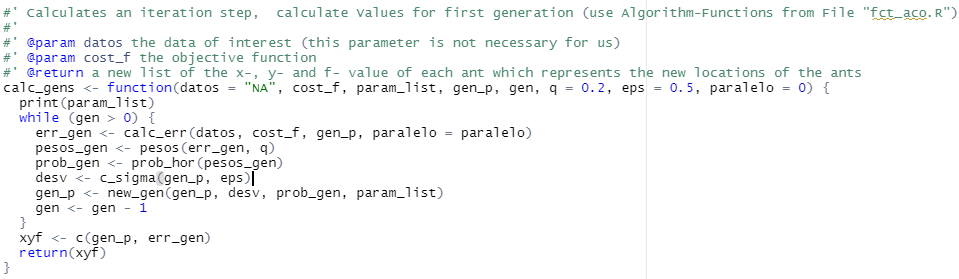
\includegraphics[scale=0.7]{"images/04_Visualisierung_des_Algorithmus/util_makeNewGen.png"}
 \caption{Definition von Funktionen in global\_utils.R um einen Iterationsschritt des ACO durchzuführen}
 \label{fig:util_makeNewGen}
\end{figure}

Um die Ameisenwerte, deren Mittelwert und die tatsächlichen Minima der Himmelblaufunktion graphisch darstellen zu können, werden die Werte in einer weiteren Funktion vorbereitet. Hierzu wird ein DataFrame erstellt, das neben den Spalten für die Koordinaten der Punkte eine zusätzliche Spalte besitzt, mithilfe welcher den Punkten eine Kategorie zugewiesen wird. Diese bestimmt, ob es sich bei dem Wert um einen Ameisenwert, einen Mittelwert oder ein tatsächliches Minimum handelt. Die Spalte wird benötigt, um den Punkten im Graphen je nach Kategorie unterschiedliche Farben verleihen zu können.
Die Deklaration dieser vorbereitenden Funktion zeigt Abbildung \ref{fig:util_prepareForPlot}.


\begin{figure}[H]
 \centering
 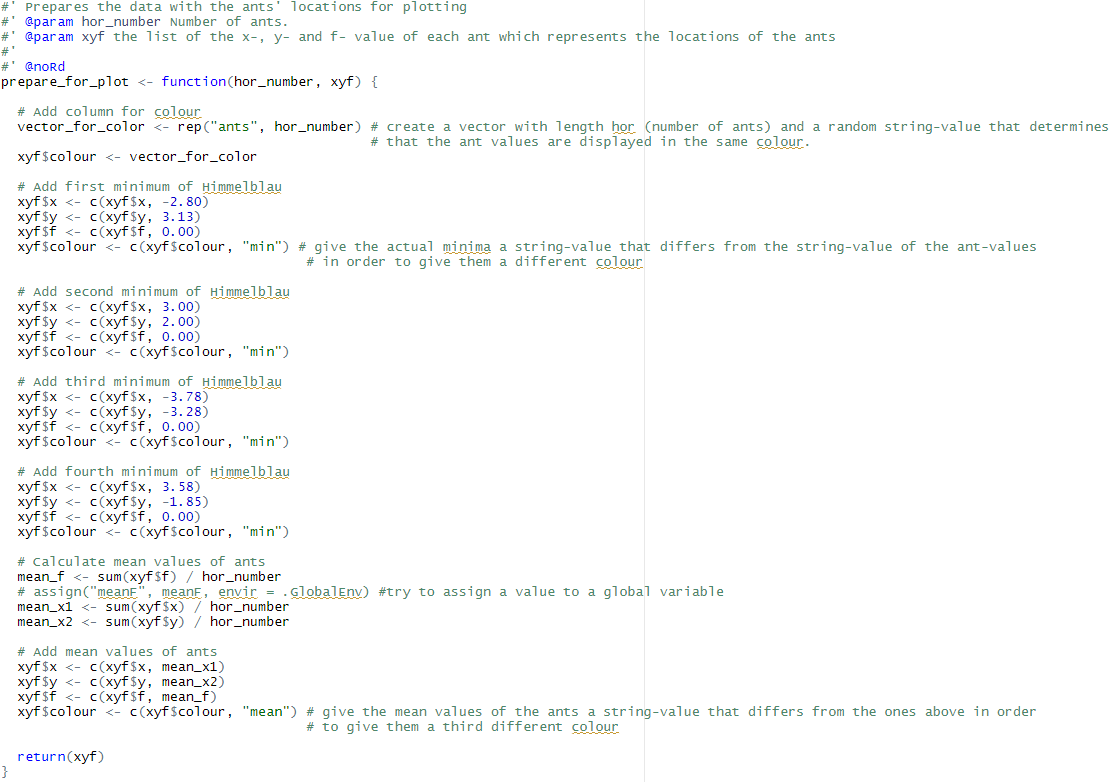
\includegraphics[scale=0.6]{"images/04_Visualisierung_des_Algorithmus/util_prepareForPlot.png"}
 \caption{Definition einer Funktionen in global\_utils.R um die Ameisenwerte, deren Mittelwert und die tatsächlichen Minima in einem Data Frame zu speichern, um sie in einem Graph darstellen zu können}
 \label{fig:util_prepareForPlot}
\end{figure}

Aufgerufen werden die genannten Funktionen in einem output-Element der \linebreak mod\_ant\_generations\_tab.R Datei (siehe Abbildung \ref{fig:antGenerations_plotGens}). Ebenfalls wird hier die Reaktivität der Parameter auf Benutzereingaben umgesetzt und der Graph dargestellt. 
Da das dreidimensionale Punktediagramm unter Verwendung des R-Pakets plotly erstellt wird, ist dessen Ansicht per Mausziehen verschiebbar und die Koordinaten eines Punkts werden angezeigt, sobald der Benutzer mit dem Mauszeiger darüber schwebt.
Dem Benutzer wird deutlich, dass sich der Algorithmus mit steigender Anzahl an Ameisen und Iterationen, einem der Minima nähert.  Wie vorhergehend erläutert, kann auch hier kein Kriterium identifiziert werden, das bestimmt, in welches der Minima der Algorithmus konvergiert.


\begin{figure}[H]
 \centering
 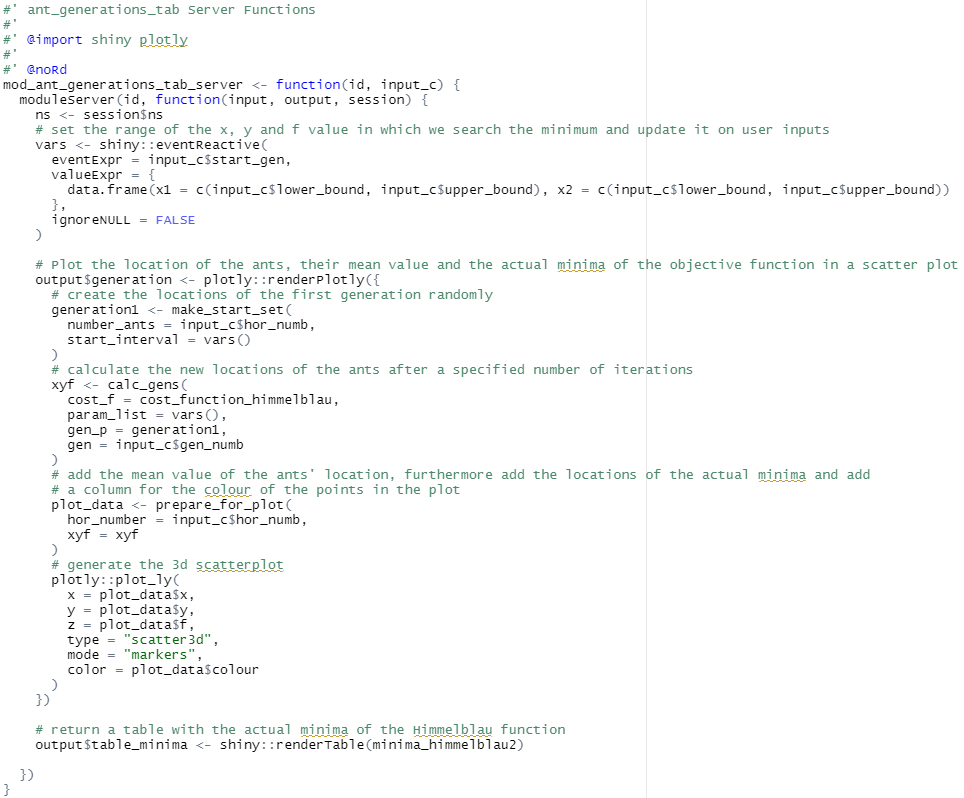
\includegraphics[scale=0.7]{"images/04_Visualisierung_des_Algorithmus/antGenerations_plotGens.png"}
 \caption{Server-Output Elemente der mod\_ant\_generations\_tab.R Datei um den Suchbereich zu aktualisieren, Ameisengenerationen zu berechnen und graphisch darzustellen}
 \label{fig:antGenerations_plotGens}
\end{figure}
	\section{Das Problem des Handlungsreisenden als Beispielanwendungsfall}\label{chap:TSP}

Dieser Algorithmus wird heute immer noch häufig für verschiedene Problemstellungen verwendet. Bekannte Anwendungsfälle sind \citep[S.9]{Blum2003}:
\begin{itemize}
  \item Busrouten, Müllabfuhr, Post- und Auslieferungsrouten
  \item Maschinenbelegungsproblem: Minimierung der Transportzeit bei räumlich weit auseinander liegenden Produktionsstätten
  \item Routenoptimierung zur Nachschubversorgung von Fertigungslinien mit minimalem Transportmitteleinsatz 
  \item 2D HP Proteinfaltung
  \item Beschickung von Lackieranlagen
  \item Fertigungssteuerung
  \item Telefonnetzwerk und Internet
  \item Personaleinsatzplanung
  \item Optimale Steuerung und Auslastung von Fahrzeugen und Fahrwegen
  
\end{itemize}
Ein sehr bekannter Anwendungsfall ist das Traveling Salesman Problem. Hierbei geht es um eine Optimierung in dem Bereich der Routenoptimierung. Ein Händler möchte mehrere Städte in so kurzer Zeit wie möglich besuchen und dann wieder zu seinem Ausgangspunkt zurückkehren \citep[S.37]{OKWU.2021}.
\newline
\newline
Dieses Problem wird auch in dem Shiny-Dashboard dargestellt und gezeigt, wie sich die Ergebnisse bei verschiedenen Einstellungen der Parameter ändert. Die Anzahl und die Orte der Städte bleiben dabei immer gleich, sodass man die Unterschiede durch die Parameter direkt sehen kann.
\newline
Auf dem Dashboard sieht man ein Koordinatensystem mit mehreren Slidern an der Seite und zwei ActionButtons. Die Funktionen für den Plot, die Slider und die Buttons werden in dem SKript mod-tsp-tab festgelegt. Auch die Server Funktionen sind in diesem Skript zu finden.
\begin{figure}[H]
 \centering
 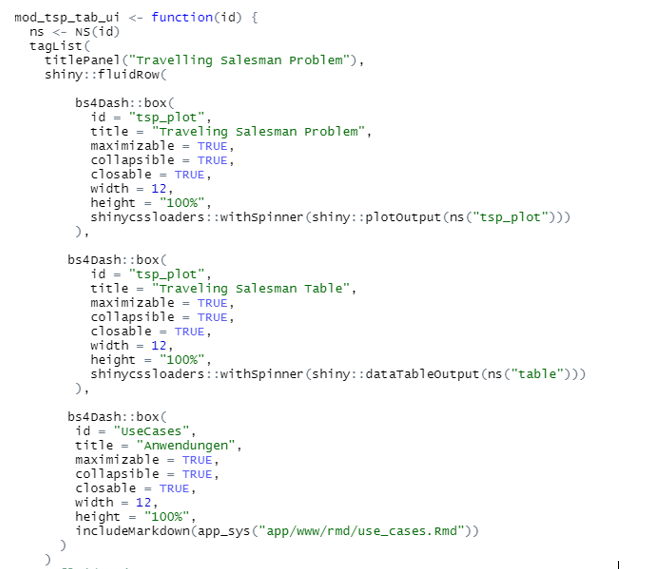
\includegraphics[scale=.7]{"images/05_Tsp/ui_mod_tsp_tab.png"}
 \caption{Quellcode für die UI Funktion des TSP Tabs}
 \label{fig:ui_mod_tsp_tab}
\end{figure}

\begin{figure}[H]
 \centering
 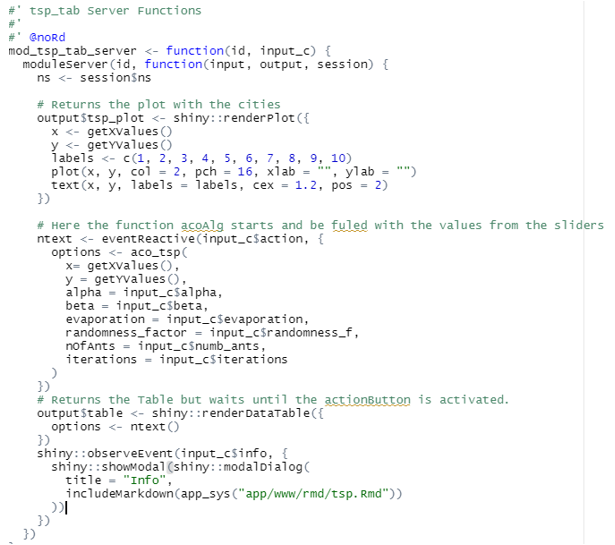
\includegraphics[scale=.7]{"images/05_Tsp/server_mod_tsp_tab.png"}
 \caption{Quellcode für die Server Funktion des TSP Tabs}
 \label{fig:server_mod_tsp_tab}
\end{figure}
Die erste Funktion im Server: output\$TSPlot ist zuständig für die Ausgabe des Plots.
\newline 
In unserem Beispiel wird mit 10 Städten gerechnet. Die X-, und Y-Werte werden über die Funktionen getXValues() und getYValues() gezogen. Diese Werte bleiben auch immer gleich. Mit der Abbildung kann man selbst immer die ausgegebenen Wege des ACO-Algorithmus nachgehen und entscheiden, ob die Lösung des Algorithmus eine Gute ist oder nicht.
\newline
In dem Shiny-Dashboard kann der Benutzer selbständig die Parameter über mehrere Slider an der Seite bestimmen und über einen Action-Button die Funktion des ACO mit den Slider-Parametern aufrufen. In der Funktion ntext <- eventReactive() wird der ACO mit den Werten der Slider befüllt und dann aufgerufen. Es werden wieder die X-, und Y-Werte mit den zwei Funktionen übergeben. Der Algorithmus wartet mit dem Aufruf der Funktion solange, bis der Benutzer auf den ActionButton klickt. 
\newline 
Im Folgenden wir dann das Ergebnis berechnet und über eine Tabelle ausgegeben, die immer alle minimalen Ruten enthält. Dabei kommt es häufig vor, dass der Algorithmus das minimale Ergebnis nicht nur einmal, sondern öfters findet und dann auch in der Tabelle ausgibt. Die Tabelle wird im Server in der Funktion output\$table <- renderDataTable() aufgerufen, sobald der ACO seine Berechnungen erledigt hat. Anhand der Distance in der Tabelle kann man sehen, ob der Algorithmus eine bessere oder schlechtere Route gefunden hat als davor.
\begin{figure}[H]
 \centering
 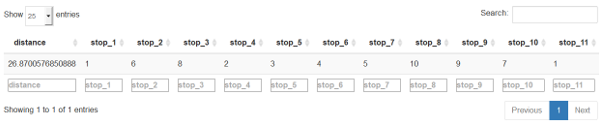
\includegraphics[scale=.7]{"images/05_Tsp/tsp_tabelle.png"}
 \caption{Tabelle mit den Ergebnissen des TSP}
 \label{fig:tsp_tabelle}
\end{figure}
Die Slider, der Plot und die Tabelle werden in der UI festgelegt und mit Min-, Max- und Anfangswerten versehen. Die Intervalle der Slider kann man dadurch schnell anpassen und auch größere Rechnungen durchführen, wenn man das möchte. Für die größeren Rechnungen muss man auch mehr Zeit einplanen. Hier ist der Action Button wichtig, der für die Ausführung des ACO -Algorithmus zuständig ist. Ohne ihn würde der Algorithmus bei jeder Änderung eines Slider und direkt beim Starten des Dashboards ausgeführt werden, das führt dann zu langen Wartezeiten und man kann nicht mehrere Parameter für seine Versuche mit dem Algorithmus verändern. 
\newline
\newline
Der Algorithmus, der das TSP durchführt ist von dem  \href {https://github.com/ciessielski/ACOTSP} {Git-Repository}. Dabei wurden kleine Änderungen gemacht, wie das Verändern der festen Parameter über die Slider. 
\newline
Der ACO Algorithmus wird über die Funktion aco-tsp ausgeführt.
\begin{figure}[h]
 \centering
 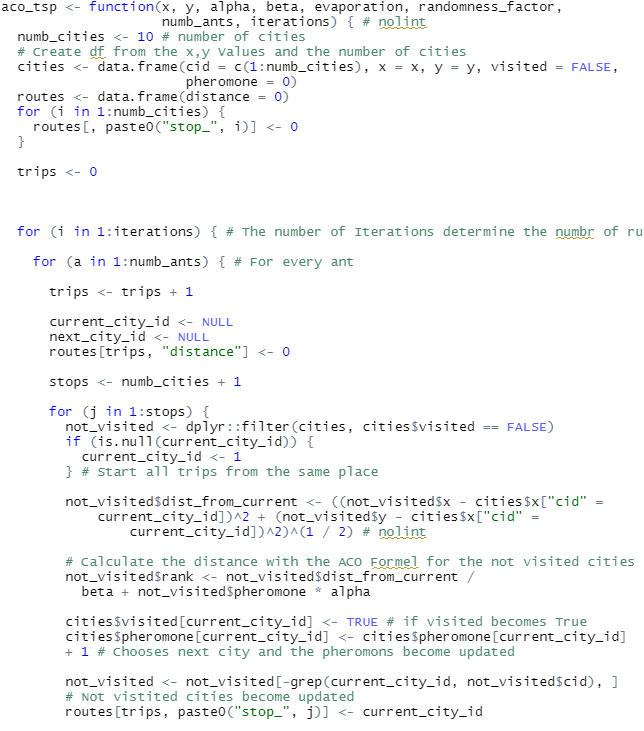
\includegraphics[scale=.6]{"images/05_Tsp/fct_aco_tsp1.png"}
 \caption{Quellcode zu TSP ACO Function}
 \label{actionButtonPhasen}
\end{figure}
\begin{figure}[h]
 \centering
 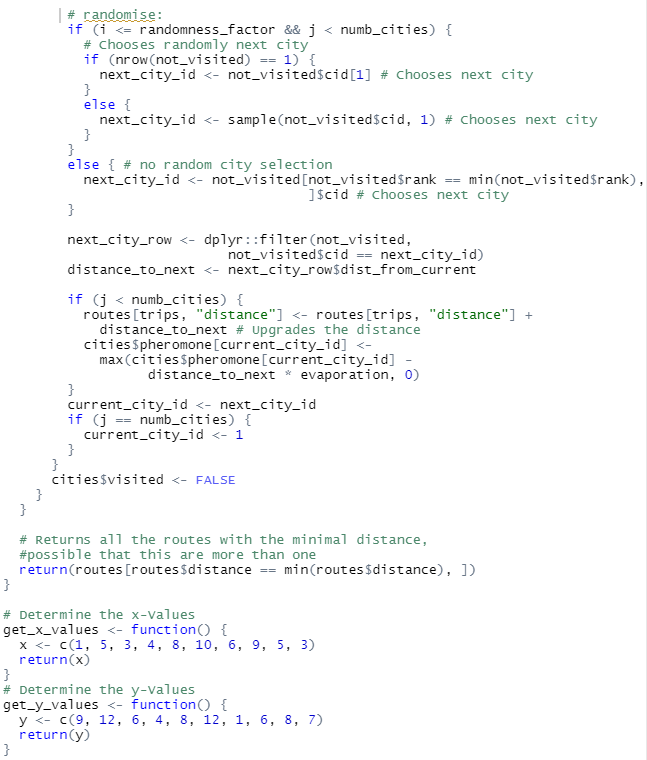
\includegraphics[scale=.6]{"images/05_Tsp/fct_aco_tsp2.png"}
 \caption{Quellcode zu TSP ACO Function}
 \label{actionButtonPhasen}
\end{figure}

Am Anfang des Codes werden die Parameter übergeben und ein Data Frame aus den X- und Y-Werten erstellt. Anhand der Anzahl der Städte wird die Anzahl an Stopps berechnet. Diese muss um eins höher sein als die Anzahl der Städte.
\newline
Für jede angegebene Iteration werden nun die einzelnen Schritte durchgeführt. Dabei durchläuft jede Ameise einen bestimmten Durchlauf. Bei jedem Durchlauf wird eine Route erstellt. Bei jeder Route ist das Ziel eine Distanz aufzunehmen und am Ende von allen Distanzen die Minimale mit ihren Stopps in der Reihenfolge auszugeben.
\newline
Jede Ameise beginnt bei der gleichen Stadt. Das wird direkt am Anfang der For-Schleife bei den Stopps festgelegt. Danach werden alle Distanzen zu den anderen Städten berechnet und den noch nicht besichtigten Städten einen Rang gegeben. Der Rang setzt sich aus der mathematischen Formel des ACO Algorithmus von Beta, Pheromonen und Alpha zusammen. Danach wird der Status der Stadt auf besichtigt gesetzt und die nächste Stadt in der Route ausgewählt. Die Auswahl der nächsten Route kann auch zufällig passieren, je nachdem wie hoch der Randomness-factor gesetzt wurde. Nach der Auswahl der nächsten Stadt, wird die Pheromonspur der Strecke von der aktuellen Stadt und der nächsten Stadt erhöht aber auch mit der Verdunstung verrechnet. Danach wird dasselbe mit der nächsten Stadt gemacht, nur dass es diesmal eine Möglichkeit weniger gibt, die die Ameisen wählen kann, da eine Stadt nur einmal besichtigt werden kann. 
\newline
Nachdem alle Städte abgelaufen wurden, wird die nächste Ameise ausgewählt. Sobald alle Ameisen ihre Routen gelaufen sind, wird alles nochmal ausgeführt, bis die Anzahl an Iterationen erreicht ist.
\newline
Jede Tour von jeder Ameise wird dabei in einer Tabelle mit der Distanz der Ameise gespeichert. Am Ende werden dann alle Routen mit der minimalen Distanz ausgegeben. 
\newline
\newline
Der Ameisenalgorithmus findet auch heute noch seine Anwendungen und ist sehr beliebt, wenn es um das schnelle Finden von einer guten Lösung geht. Es wird aber nicht immer die beste Lösung gefunden, außerdem ist es für den ACO beinahe unmöglich, eine noch bessere Route zu finden, wenn er schon eine sehr gute gefunden hat. Das schließt dann auch die Anwendung des ACO aus, wenn die Aufgabe besteht eine genaue und ideale Lösung zu finden \citep{LogistikInfonodate}.
\newline
\newline
Weitere Nachteile des Ameisenalgorithmus sind seine Komplexität und seine Ungenauigkeit. Den Ameisenalgorithmus manuell durchzuführen ist beinahe unmöglich und daher auch nur mit einem Computer machbar. Es ist außerdem wichtig für den ACO-Algorithmus, dass die Probleme als Graphen dargestellt werden müssen, damit Lösungen konstruierbar sind.
\newline
\newline
Trotz allem wird der Ameisenalgorithmus sehr gerne in der Logistik angewandt, da dort eine gute Lösung sehr häufig reicht, um sehr viel Geld oder Zeit zu sparen. Es ist daher in der Logistik nicht notwendig, immer die beste Lösung zu finden \citep{LogistikInfonodate}.

	\section{Performancevergleich mit anderen Algorithmen}\label{chap:Performance}

In der Metaheuristik existieren eine Vielzahl evolutionärer Algorithmen (EAs)\nomenclature{EAs}{evolutionäre Algorithmen}. Alle basieren auf der biologischen Evolution und/oder dem sozialen Verhalten einer Spezies und ermöglichen es komplexe Optimierungsprobleme zu lösen, welche zum Teil mit herkömmlichen Methoden nicht lösbar sind. \newline
In dem vorliegenden Dashboard wurde der ACO Algorithmus verschiedenen weiteren EA Algorithmen im Hinblick auf die Qualität der Ergebnisse gegenübergestellt. \newline 
Alle Algorithmen lösen dabei ein Minimierungsproblem auf entweder der Himmelblau- oder der Rosenbrockfunktion. Es werden ausschließlich zwei Parameter (x1, x2), sowie ein diskreter Zahlenraum betrachtet.\newline 
Der Zahlenraum (untere und obere Grenze), sowie die Anzahl an Evolutionen und die Populationsgröße können konfiguriert werden, um die Auswirkung der verschiedenen Parameter auf die Ergebnisse der Algorithmen zu sehen. \newline 
Folgende Algorithmen werden im Dashboard gegenübergestellt: 
\begin{itemize}
    \item Ant Colony Optimization Algorithm
    \item Ant Lion Optimization Algorithm 
    \item Bat Optimization Algorithm 
    \item Cat Swarm Optimization Algorithm
    \item Dragonfly Optimization Algorithm 
    \item Firefly Optimization Algorithm 
\end{itemize}
Der oder die am besten abschneidenden Algorithmen werden nach Abschluss der Berechnung grün, der am schlechtesten abschneidene Algorithmus rot und die Anderen gelb hervorgehoben.
\begin{figure}[H]
 \centering
 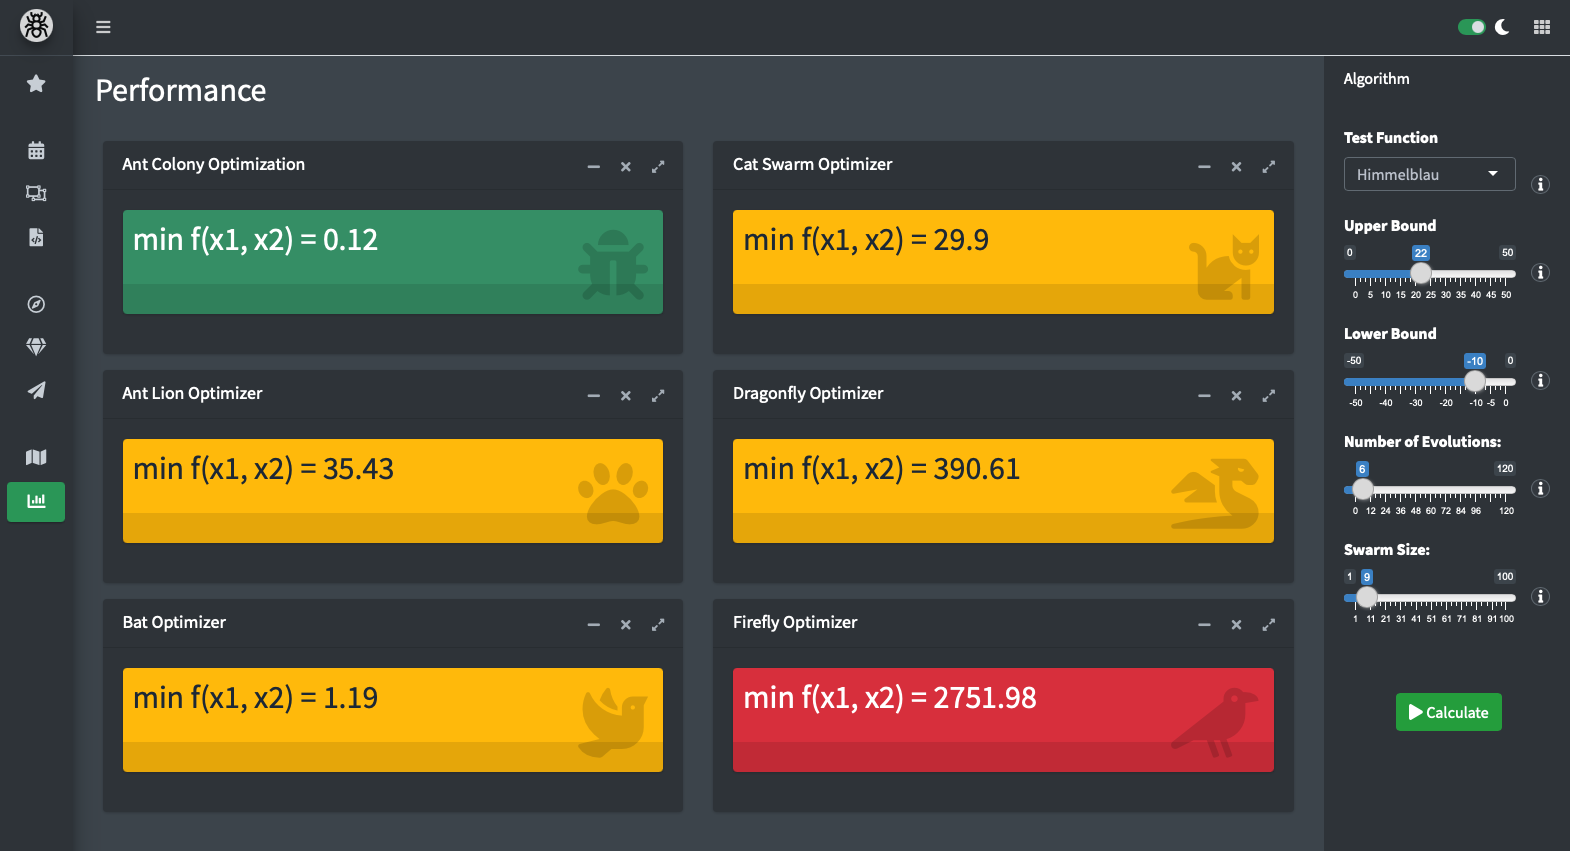
\includegraphics[scale=0.2]{"images/06_Performancevergleich/performance_tab.png"}
 \caption{Performance Tab mit farblicher Hervorhebung der Ergebnisse der einzelnen Algorithmen}
 \label{fig:performance_tab}
\end{figure}

Die Implementation der einzelnen EA Algorithmen, mit Ausnahme des ACO Algorithmus basieren auf dem Paket \emph{metaheuristicOpt} \citep{Riza2019}. Ein Paket, welches verschiedenste metaheuristische Optimierungsalgorithmen implementiert. \newline 
Die Implementation des ACO Algorithmus basiert auf dem Paket evoper \cite{Garcia2018}.
Der Performance Tab ist wie folgt designed: Er besteht aus sechs bs4Dash Karten, welche selber nochmal valueBoxen enthalten. Diese valueBoxen werden vom Server aus befüllt. Dabei sind Informationen, wie das Icon oder der erste Teil des Headers statisch, die Color Property und der zweite Teil des Headers dynamisch. \newline 
Die Controlbar, welche die Input Elemente zum Konfigurieren der Algorithmen enthält ist nicht in dem mod\_performance\_tab.R Modul, sondern in der fct\_update\_controlbar.R Datei enthalten. Diese Funktion updated den Inhalt der Controlbar abhängig von gerade ausgewählten Tab und muss folglich global und nicht in einem Modul implementiert sein. \newline 

\begin{figure}[h]
 \centering
 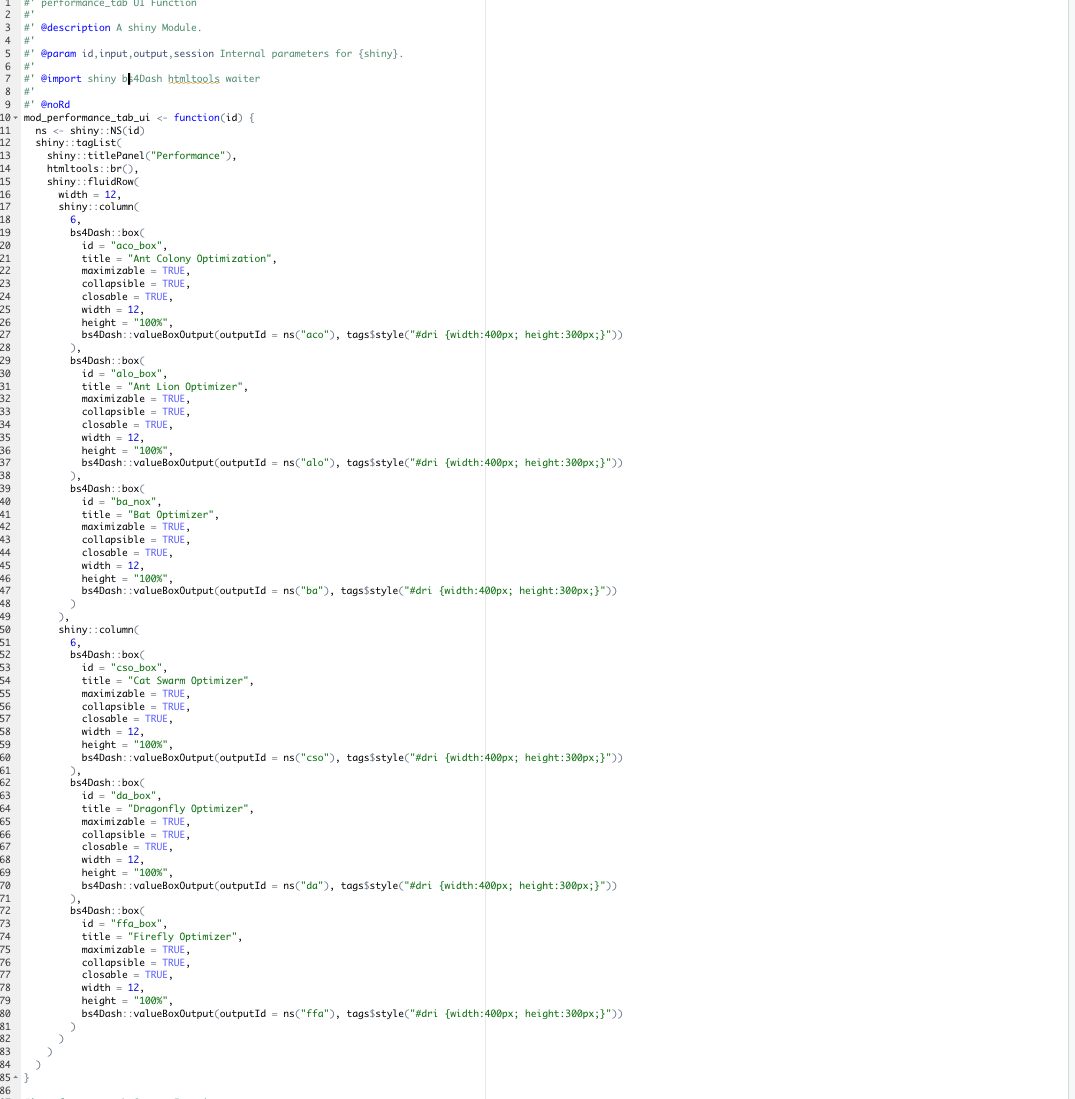
\includegraphics[scale=0.4]{"images/06_Performancevergleich/ui_performance_tab.png"}
 \caption{UI Funktion des Performance Tabs}
 \label{fig:ui_performance_tab}
\end{figure}

\begin{figure}[H]
 \centering
 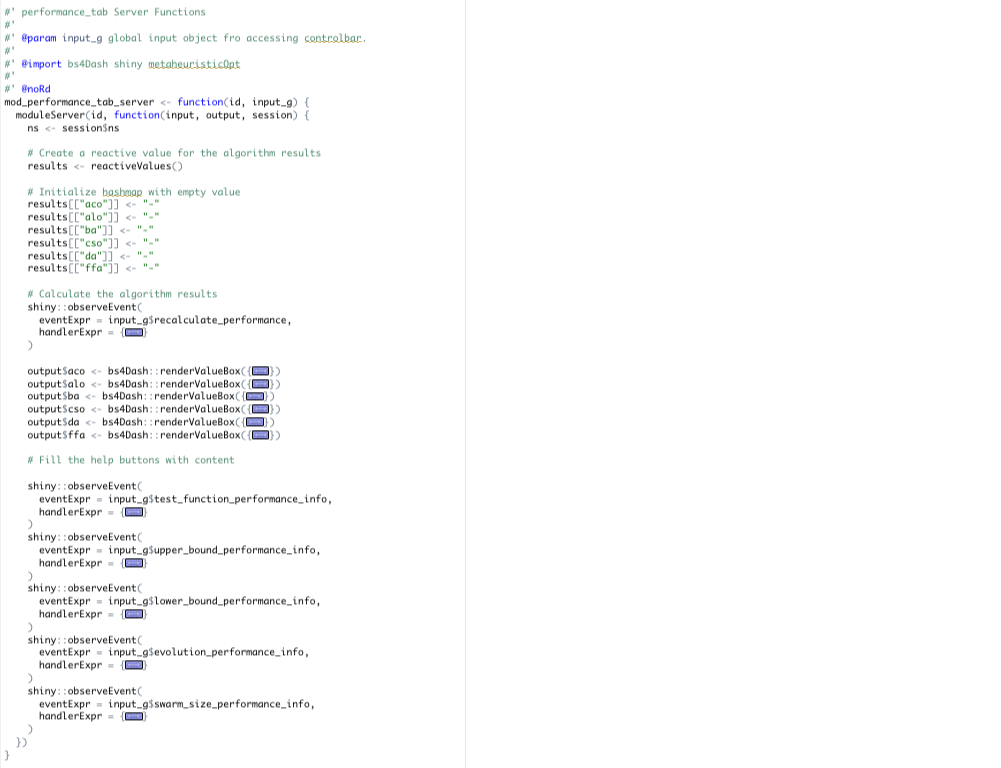
\includegraphics[scale=0.4]{"images/06_Performancevergleich/server_performance_tab.png"}
 \caption{Server Funktion des Performance Tabs mit eingeklappten Funktionen}
 \label{fig:server_performance_tab}
\end{figure}

Abschließend gilt es die get\_color Funktion zu erwähnen. Diese updated die valueBox Farbe, abhängig vom Ergebnis des Algorithmus. Die Logik basiert dabei auf der Idee, dass die Mimima der Rosenbrock- und Himmelblau Funktion jeweils bei y=0 liegen. Umso dichter also die in die Kostenfunktion eingesetzten Funktionswerte an Null sind, umso besser perfomt der Algorithmus. 
\begin{figure}[H]
 \centering
 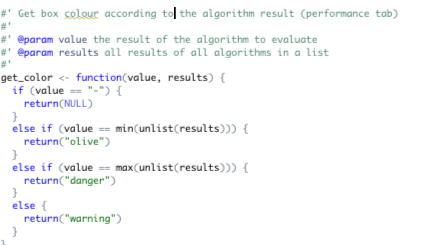
\includegraphics[scale=0.4]{"images/06_Performancevergleich/utils_get_color.png"}
 \caption{get\_color Funktion, welche die Box-Farbe abhängig vom Ergebnis des Algorithmus updated}
 \label{fig:server_performance_tab}
\end{figure}
	\section{Fazit}\label{chap:Fazit}
Zusammenfassend kann gesagt werden, dass sich ein R-Shiny Dashoard gut eignet, um ein Optimierungsverfahren zu präsentieren und die Herkunft, Wirkungsweise, Anwendungsbeispiele und Performance eines Algorithmus anschaulich darzustellen. Mit relativ einfachen Mitteln kann mit R-Shiny ein ansprechendes und übersichtliches Dashboard erstellt werden, das dem Benutzer einen Überblick über wichtige Aspekte des Algorithmus gibt.\newline
Als besonders sinnvoll erweist sich hierbei die Verwendung interaktiver Elemente. \newline
Durch diese kann dem Benutzer beispielsweise die Möglichkeit gegeben werden, Parametereinstellungen des Algorithmus zu ändern, die sich auf das Ergebnis auswirken, wodurch der Benutzer die Auswirkungen von Parameteränderungen auf das Ergebnis selbst beliebig erproben kann. 
Indem der Benutzer bei der Benutzung des Dashboards aktiv sein kann, erhöht sich folglich sein Interesse und der Lerneffekt.  
Indem auf ein durchgehend schlichtes Design geachtet wird und überfüllte Ansichten vermieden werden, wird zudem erreicht, dass klar verständlich ist, welcher Inhalt relevant ist und der Fokus auf dem Wesentlichen liegt.


    \section{Kennzeichnung der Anteile der Studierenden}

Markus Koch:
\begin{itemize}
\item \nameref{chap:Einleitung}, \nameref{chap:Fazit}
\item \nameref{chap:Aufbau}
\item \nameref{chap:Einordnung}
\item \nameref{chap:VerhaltenAmeisen}
\end{itemize}

Moritz Link: 
\begin{itemize}
\item \nameref{chap:Geschichte}
\item \nameref{chap:TSP}
\end{itemize}

Felix Behne:
\begin{itemize}
\item \nameref{chap:Golem}
\item \nameref{chap:Performance}
\end{itemize}

Sarah Engelmayer: 
\begin{itemize}
\item \nameref{chap:Formeln}
\item \nameref{chap:Visualisierung}
\end{itemize}

    
	% Anhang
	\renewcommand{\thetable}{\Alph{section}.\arabic{table}}              % Tabellennummerierung mit Section
	\renewcommand{\thefigure}{\Alph{section}.\arabic{figure}}            % Abbildungsnummerierung mit Section
	\renewcommand{\thelstlisting}{\Alph{section}.\arabic{lstlisting}}    % Listingsnummerierung mit Section
	
	\begin{appendix}
	%\include{chapter/30_anhang}
	\end{appendix}
	
	% Abschluss
	\bibliography{literatur/literatur}
\newpage

	\renewcommand{\indexname}{Stichwortverzeichnis}
\printindex
\newpage

	\thispagestyle{empty}
\addcontentsline{toc}{section}{Selbständigkeitserklärung}
\begin{center}
	\vspace*{2cm}
	\Huge\bf Selbständigkeitserklärung\\
	\vspace*{3cm}
	\normalsize\rm
    Wir versichern hiermit, dass wir den Projektbericht \fi ~mit dem Thema\\
	\vspace*{2cm}
	\Large\bf\myTopic\\
	\Large\rm\mySubTopic\\
	\vspace*{2cm}
	\normalsize\rm
	selbständig verfasst und keine anderen als die angegebenen\\Quellen und Hilfsmittel benutzt haben.\\
	Zudem versichern wir, dass die eingereichte
	elektronische Fassung mit der gedruckten Fassung übereinstimmt.\\
	\vfill
	\begin{tabularx}{\textwidth}{l@{\extracolsep\fill}r}
  	\rule{7cm}{0.3mm}&\rule{7.55cm}{0.3mm}\\
	\end{tabularx}
	\begin{tabularx}{\textwidth}{*{2}{>{\arraybackslash}X}}
	  Ort, Datum&Unterschrift Felix Behne\\
	\end{tabularx}
	\begin{tabularx}{\textwidth}{l@{\extracolsep\fill}r}
		\rule{7cm}{0.3mm}&\rule{7.55cm}{0.3mm}\\
	\end{tabularx}
	\begin{tabularx}{\textwidth}{*{2}{>{\arraybackslash}X}}
	  Ort, Datum&Unterschrift Markus Koch\\
	\end{tabularx}
	\begin{tabularx}{\textwidth}{l@{\extracolsep\fill}r}
		\rule{7cm}{0.3mm}&\rule{7.55cm}{0.3mm}\\
	\end{tabularx}
	\begin{tabularx}{\textwidth}{*{2}{>{\arraybackslash}X}}
	  Ort, Datum&Unterschrift Moritz Link\\
	\end{tabularx}
	\begin{tabularx}{\textwidth}{l@{\extracolsep\fill}r}
		\rule{7cm}{0.3mm}&\rule{7.55cm}{0.3mm}\\
	\end{tabularx}
	\begin{tabularx}{\textwidth}{*{2}{>{\arraybackslash}X}}
	Ort, Datum&Unterschrift Sarah Engelmayer\\
    \end{tabularx}
\end{center}

\end{document}

%%%%%%%%%%%%%%%%%%%%%%%%%%%%%%%%%%%%%%%%%%%%%%%%%%%%%%%%%%%%%%%%%%%%%%%%%%%%%
%%                                                                         %%
%% /\   /\         Ab hier keine Änderungen mehr vornehmen         /\   /\ %%
%%                                                                         %%
%%%%%%%%%%%%%%%%%%%%%%%%%%%%%%%%%%%%%%%%%%%%%%%%%%%%%%%%%%%%%%%%%%%%%%%%%%%%%